\begin{frame}
\begin{center}

\includegraphics[scale=0.40]{img/noidea.jpg}

Je dis une connerie $\Rightarrow$ interrompez moi !
\end{center}
\end{frame}

\subsection{Structure des fichiers}

\begin{frame}{/}
\begin{description}
  \item [app] Le dossier ou le code de l'application CakePHP est placé (notre dossier de travail)
  \item [lib] Le dossier où le code de CakePHP est placé
  \item [vendors] Autres bibliothèques PHP
  \item [plugins]
  \item [.htaccess]
  \item [index.php]
  \item [README]
\end{description}
\end{frame}

\begin{frame}{/app/}
\begin{description}
  \item [Config] Les fichiers de configuration y sont placés
  \item [Console] Les commandes pour la console
  \item [Controller] Les controlleurs du motif MVC
  \item [Lib] Classes ou bibliothèques CakePHP d'origine interne
  \item [Locale] Internationalisation
  \item [Model] Le modèle du motif MVC
  \item [Plugin] Des plugins...
  \item [Test] Contient des cas de test (pour tester le bon fonctionnement de l'application)
  \item [tmp] Utilisé par CakePHP pour stocker des données temporairement
  \item [Vendor] Classes ou bibliothèques CakePHP d'origine tierce
  \item [View] La vue du motif MVC
  \item [webroot] Utilisé comme racine pour les documents produits, les fichiers CSS, JavaScript ou image doivent être placés ici
\end{description}
\end{frame}

\begin{frame}
\begin{center}
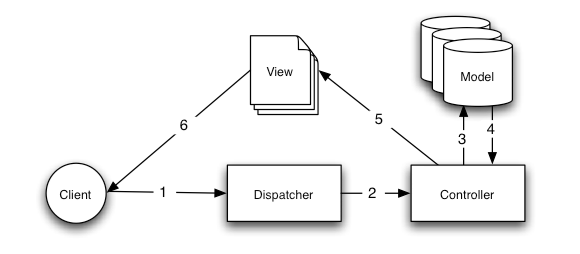
\includegraphics[scale=0.50]{img/basic_mvc.png}

\begin{enumerate}
  \item Ouverture de page par un client
  \item Le répartisseur envoie la reqête au contrôleur concerné
  \item Le contrôleur exécute la logique spécifique de l’application et demande des données au modèle
  \item Le modèle retourne les données demandées et le contrôlleur travaille avec
  \item Le contrôlleur envoie les données à la vue
  \item La vue formatte les données pour l'utilisateur et les lui retourne
\end{enumerate}
\end{center}
\end{frame}

\begin{frame}[fragile]{app/controllers/users\_controller.php}
\begin{lstlisting}[language=c++]
<?php
class UsersController extends AppController {
  var $name='Users';
  function index() {
  }
}
?>
\end{lstlisting}
\end{frame}

\begin{frame}[fragile]{app/models/user.php}
\begin{lstlisting}[language=c++]
<?php
class User extends AppModel {
  var $name='User';
}
?>
\end{lstlisting}
\end{frame}

\begin{frame}[fragile]{index.ctp}
\begin{lstlisting}[language=c++]
<html>
<?php
  echo "Hello World";
?>
</html>
\end{lstlisting}
\end{frame}

\end{document}

